%\documentclass[12pt,a4paper]{hsrthesis}
\documentclass[ngerman, a4paper,12pt]{hsrthesis}
\usepackage{babel}
\nonstopmode

\usepackage{listings}

\usepackage{graphicx, color}
\usepackage[utf8]{inputenc}


\definecolor{olivegreen}{rgb}{0.33, 0.42, 0.18}
\usepackage{attachfile}
\usepackage{dirtytalk}

\sffamily


\lstset{
    	frame=single,
    	breaklines=true,
	basicstyle=\footnotesize,
    	postbreak=\raisebox{0ex}[0ex][0ex]{\ensuremath{\color{red}\hookrightarrow\space}},
    	morecomment=[l][\color{olivegreen}]{\#},
	morestring=[b][\color{blue}]\",
morekeywords={SELECT,CONSTRUCT,DESCRIBE,ASK,WHERE,FROM,NAMED,PREFIX,BASE,OPTIONAL,FILTER,GRAPH,LIMIT,OFFSET,SERVICE,UNION,EXISTS,NOT,BINDINGS,MINUS,a},
sensitive=true
}

%\usepackage[showframe]{geometry}
%\usepackage[ngerman]{babel}
           
\usepackage{csquotes}
\usepackage{graphicx}
\usepackage[acronyms]{glossaries}
\usepackage{a4wide}


\makeindex

% do this here, so you can \gls{...} to it
%add new glossaryentries here...

\newglossaryentry{sqlite}{
	name=SQLite,
	description={SQLite ist eine Datenbankengine, welche ohne Konfiguration auskommt. Es handelt sich dabei um eine Datenbank in einer Datei},
	first={SQLite}
}

\newacronym{srid}{SRID}{Spatial Reference Identifier}

\newacronym{srid}{GIS}{Geografische Informationssystem}
\makeglossaries

\begin{document}
\sffamily
\setlength{\oddsidemargin}{0mm} 
\setlength{\evensidemargin}{0mm}

\newcommand{\thesistitle}{Waldmeister - Outdoors}
\newcommand{\thesissubtitle}{Ein Werkzeug zur Erfassung und Publikation von Waldstandorten}
\newcommand{\thesisauthora}{Daniel Schmider}
\newcommand{\thesisauthorb}{}
\newcommand{\thesisauthorc}{}
\newcommand{\professor}{Prof. Stefan Keller}
\newcommand{\thesistype}{Projektarbeit 2}
\newcommand{\departement}{Master of Science in Engineering, Major Software and Systems}
\newcommand{\school}{HSR Hochschule für Technik Rapperswil}
\newcommand{\term}{Fall 2017}
\newcommand{\thedate}{}
\newcommand{\timeperiode}{21.09.2017 - 01.03.2018}

\setlength{\oddsidemargin}{0mm}
\maketitle
%\setlength{\oddsidemargin}{20mm}



\renewcommand\thesection{\arabic{section}}
%03introduction.tex

\chapter{Abstract}
"Waldmeister-Outdoors" ist eine Applikation, welche es erm\"oglicht, Waldstandorte in der Schweiz zu erforschen und zu erfassen. \"Uber eine Webapplikation k\"onnen sich Benutzer Registrieren und \"offentliche, bzw. private Benutzerfl\"achen von mehreren Ger\"aten aus zu erstellen, speichern und teilen. Diese k\"onnen Waldstandorte, aber auch zus\"atzliche relevante Informationen zu einem Standort beinhalten. "Waldmeister-Outdoors" erleichtert die digitale Erfassung und Publikation von Waldstandorten und kann Experten die Arbeit im Feld erleichtern. Mithilfe der Geolocation wird der eigene Standort bestimmt und umliegende, bereits erfasste Waldstandorte und Benutzerfl\"achen werden auf einer Karte angezeigt.
$\newline$
\textbf{Keywords: Vue.JS, Django, Rest Framework, Leaflet, Leaflet editable, Geolocation, Progressive Webapp} 









\tableofcontents


% The main content
%%%%%%%%%%%%%%%%%%
%\chapter*{Examples}

\section*{Glossary Example}

\gls{sqlite} ist ein Glossar Eintrag. Lorem ipsum dolor sit amet, consetetur sadipscing elitr, sed diam nonumy eirmod tempor invidunt ut labore et dolore magna aliquyam erat, sed diam voluptua. At vero eos et accusam et justo duo dolores et ea rebum.

\section*{Bibliography and Citation Example}

Dies ist ein Zitat aus einem Buch\cite{Matthews201111}. Lorem ipsum dolor sit amet, consetetur sadipscing elitr, sed diam nonumy eirmod tempor invidunt ut labore et dolore magna aliquyam erat, sed diam voluptua. At vero eos et accusam et justo duo dolores et ea rebum.

Lorem ipsum dolor sit amet, consetetur sadipscing elitr, sed diam nonumy eirmod tempor invidunt ut labore et dolore magna aliquyam erat, sed diam voluptua. At vero eos et accusam et justo duo dolores et ea rebum. Stet clita kasd gubergren, no sea takimata sanctus est Lorem ipsum dolor sit amet. Lorem ipsum dolor sit amet, consetetur sadipscing elitr, sed diam nonumy eirmod tempor invidunt ut labore et dolore magna aliquyam erat, sed diam voluptua. At vero eos et accusam et justo duo dolores et ea rebum. Stet clita kasd gubergren, no sea takimata sanctus est Lorem ipsum dolor sit amet. Lorem ipsum dolor sit amet, consetetur sadipscing elitr, sed diam nonumy eirmod tempor invidunt ut labore et dolore magna aliquyam erat, sed diam voluptua. At vero eos et accusam et justo duo dolores et ea rebum. Stet clita kasd gubergren, no sea takimata sanctus est Lorem ipsum dolor sit amet. 

Duis autem vel eum iriure dolor in hendrerit in vulputate velit esse molestie consequat, vel illum dolore eu feugiat nulla facilisis at vero eros et accumsan et iusto odio dignissim qui blandit praesent luptatum zzril delenit augue duis dolore te feugait nulla facilisi. Lorem ipsum dolor sit amet, consectetuer adipiscing elit, sed diam nonummy nibh euismod tincidunt ut laoreet dolore magna aliquam erat volutpat. 

Ut wisi enim ad minim veniam, quis nostrud exerci tation ullamcorper suscipit lobortis nisl ut aliquip ex ea commodo consequat. Duis autem vel eum iriure dolor in hendrerit in vulputate velit esse molestie consequat, vel illum dolore eu feugiat nulla facilisis at vero eros et accumsan et iusto odio dignissim qui blandit praesent luptatum zzril delenit augue duis dolore te feugait nulla facilisi. 


\section*{Table Examples}
\subsection*{Automagical Column Widths}
\begin{tabularx}{\textwidth}{X X X X} \beforeheading
\heading{Heading 1} & \heading{Heading 2} & \heading{Heading 3} & \heading{Heading 4} \\\afterheading
Cell 1,1 & Cell 1,2 & Cell 1,3 & Cell 1,4 \\\normalline
Cell 2,1 & Cell 2,2 & Cell 2,3 Vel illum dolore eu feugiat nulla facilisis at vero eros et accumsan et iusto odio dignissim qui blandit praesent luptatum zzril delenit augue duis dolore te feugait nulla facilisi. & Cell 2,4 \\\normalline
Cell 3,1 Duis autem vel eum iriure dolor in hendrerit in vulputate velit esse molestie consequat. & Cell 3,2 & Cell 3,3 & Cell 3,4 \\\lastline
\end{tabularx}

\subsection*{Column Alignment \& Filler}
\begin{tabularx}{\textwidth}{l c r X} \beforeheading
\heading{Left Aligned} & \heading{Centered} & \heading{Right Aligned} & \heading{Filler} \\\afterheading
Cell 1,1 & Cell 1,2 & Cell 1,3 & Cell 1,4 Ut wisi enim ad minim veniam, quis nostrud exerci tation ullamcorper  \\\normalline
Cell 2,1 & Cell 2,2 & Cell 2,3 & Cell 2,4 Ut wisi enim ad minim veniam, quis nostrud exerci tation ullamcorper  \\\normalline
Cell 3,1 & Cell 3,2 & Cell 3,3 & Cell 3,4 Ut wisi enim ad minim veniam, quis nostrud exerci tation ullamcorper  \\\lastline
\end{tabularx}



%03introduction.tex
\renewcommand\thesection{\arabic{section}}
\chapter{Management summary}
\section{Problemstellung}
Je nach Untergrund, Bodeneigenschaften, Gel\"ande sowie Klima gedeihen in der Schweiz unterschiedliche Typen von W\"aldern. Seit einigen Jahrzehnten werden diese Typen von Experten erhoben und kartiert. Es wurden dabei verschiedene typisierte Waldstandorte festgelegt. Aktuell werden Karten, die im Auftrag der Kantone von Experten angefertigt wurden, nur in grossen Intervallen revidiert, wobei sie oft auch nicht fl\"achendeckend vorhanden sind (z.B. in den Kantonen GR, VS, BE).
Einer der Gr\"unde daf\"ur sind u.a. die hohen Kosten, die eine Analyse im Feld mit sich bringt.
Zudem ist die Erfassung und Nachf\"uhrung der Karten gepr\"agt von analogen Vorg\"angen, da die vorhandenen
technischen Ger\"ate und Programme f\"ur den Einsatz im Feld ungeeignet sind.
Daher muss von Hand Niedergeschriebenes im B\"uro oder von staatlichen Institutionen digitalisiert werden, bevor es an den
Arbeitgeber geschickt werden und sp\"ater auf kantonal isolierten Plattformen publiziert werden kann.

\section{Ziel der Arbeit}
Die Erfassung und Publikation von Waldstandorten sollte vereinfacht und beschleunigt werden. Dabei
sollen digitale Technologien eingesetzt werden wie Smartphone, GPS und Internet. Diese neuen
Instrumente sollen entsprechend geschulten Nutzern die Erfassung von Waldstandorten erm\"oglichen sowie \"offentliche und private Informationen in Form von Fl\"achen und Punkten. Auf einer Basis - Karte wird mittels GPS die eigene
Position angezeigt. Dar\"uber werden umliegende, bereits erfasste Waldstandorte, \"offentliche Fl\"achen anderer sowie die eigenen, privaten Fl\"achen dargestellt. Diese Fl\"achen k\"onnen Waldstandorte beschreiben oder aber zus\"atzliche Informationen \"uber den Standort beinhalten, z.B. eine speziell gekennzeichnete Beobachtungsfl\"ache.

\section{Ergebnisse}
Nach einer Evaluation eines Prototyps, erstellt mithilfe eines kommerziellen Produkts,
und der Erstellung von Mockups, wurde ein eigenes Webapp 'Waldmeister Outdoors' realisiert. Durch diese App kann die Arbeit der Experten erleichtert werden. Da die Waldstandort-Karte gleichzeitig im Web synchronisiert
ist, wird dar\"uber hinaus der Informationsaustausch unter allen Beteiligten erleichtert. Die Webapp wurde f\"ur mobile Ger\"ate optimiert und die gew\"unschten Funktionen wurden umgesetzt. Registrierte Benutzer k\"onnen Benutzerfl\"achen in Form von Polygonen direkt auf der angezeigten Map erstellen, mit zus\"atzlichen Informationen versehen und auf einem Server speichern.

\section{Ausblick}
Grosse Teile der Schweiz sind noch unkartiert, und viele Waldstandorte k\"onnten sich unter dem Einfluss der Klimaerw\"armung ver\"andern. Die kontinuierliche Beobachtung solcher Standorte ist Forschungsgegenstand und die Arbeit im Feld ist unerl\"asslich. "Waldmeister - Outdoors" kann im Berufsalltag sowie bei der Kommunikation mit Institutionen den Arbeitsfluss beschleunigen. Weitere Features wie die Verwendung von Plus Codes und offline-F\"ahigkeiten welche bei Verbindungsproblemen zum Einsatz kommen, bzw. Benutzerfl\"achen automatisch synchronisieren, sobald eine Verbindung besteht. Des weiteren bietet es sich an, dass sich User in Gruppen einklinken k\"onnen, um unter sich Benutzerfl\"achen zu teilen und zu besprechen, bevor sie ver\"offentlicht werden. Ebenfalls sollten erstellte Fl\"achen von registrierten Benutzern und deren Gruppen ver\"andert und gel\"oscht werden k\"onnen, nachdem sie erstellt wurden. $\newline$
"Waldmeister - Outdoors" hat das Potential in der Schweiz ein verbreitetes Tool zur Kartierung und Beobachtung von Waldfl\"achen zu werden und stellt eine bereits gefragte Erweiterung der beliebten "Waldmeister" App f\"ur mobile Ger\"ate dar.

\renewcommand\thesection{\thechapter.\arabic{section}}

\chapter{Teil 1 - Technischer Bericht}
\section{Einf\"uhrung}
\subsection{Problemstellung, Vision}
\subsection{Ziele und Unterziele}
\subsection{Rahmenbedingungen}
\subsection{Vorgehen, Aufbau der Arbeit}

\section{Stand der Technik}
\subsection{GIS-Browser}
Ein GIS-Browser, wie er von den verschiedenen Kanton in der Schweiz eingesetzt wird, ist ein read-only Archiv, bestehend aus �ffentlich zug�nglichen Daten. 
\subsection{ArcGIS online}
Technologien von ESRI (Environmental Systems Research Institute) und insbesondere ArcGIS (GIS; Geografisches Informationssystem) online wurden recherchiert, um einen funktionierenden Prototypen mit offline-caching zu erstellen. Hintergrundkarten (in Form eines Tile-Layers) k\"onnen auf dem Ger\"at zwischengespeichert werden. Die Erstellung von editierbaren Vektorlayern funktioniert auch beim offline Betrieb und k\"onnen sp\"ater, sobald wieder eine stabile Internetverbindung besteht, synchronisiert werden. Dieses Verhalten kann bei einer PWA durch Service-Worker rekreiert werden.$\newline$
Ein GeoJSON (Geo JavaScript Object Notation) file kann ebenfalls auf der online Plattform von ArcGIS hochgeladen werden und danach auf der Map dargestellt werden. Das Layer Styling kann so konfiguriert werden, dass die Farbe eines Polygons dem Typ des jeweiligen Waldstandorts entspricht.
\subsection{Defizite}
Ein GIS-Browser wie z.B. vom Kanton Z�rich bietet keine M�glichkeit die eigene in Betracht zu ziehen, um damit den Kartenausschnitt zu bestimmen oder genauer noch, den aktuellen Waldstandortstyp per GPS zu bestimmen. Auch ist es nicht m�glich, pers�nliche Notizen oder Fl�chen wie Beobachtungsfl�chen zu definieren, damit sie w�hrend der Arbeit im Feld verwendet werden k�nnen. Dies liegt daran, dass sich ein User nicht identifizieren kann und alle Benutzer als anonym behandelt werden.

\section{Bewertung}
\subsection{Kriterien}
\subsection{Schlussfolgerungen}

\section{Umsetzungskonzept}
\subsection{L�sungsans�tze}
\subsubsection{Backend}
\subsubsection{Frontend}
\subsubsection{Datenbank}
\subsubsection{JavaScript Libraries}
\subsubsection{Python Pakete}
\subsubsection{Werkzeuge und Tools}
\subsubsection{Testing}

\section{Resultate}
\subsection{Zielerreichung}
\subsection{Ausblick und Weiterentwicklung}
\subsection{Pers�nliche Berichte}
\subsection{Danksagungen}
\clearpage
\pagebreak


\chapter{Teil 2 - SW-Projektdokumentation}
\section{Vision}

\section{Anforderungsspezifikationen}
\subsection{Must-Haves}
\subsection{Optional}
\subsection{Use-Cases}
\subsection{Funktionale Anforderungen}
\subsection{Nicht-funktionale Anforderungen}
\subsection{Weitere Funktionen und Anforderungen}
\subsection{Detailspezifikationen}

\section{Analyse}
\subsection{Klassendiagramm}
\subsection{Domain Modell}
\subsection{Objektkatalog}

\section{Technologien}
\subsection{Django}
Als Server zur Verwaltung der User und der Daten, welche die User generieren und ben\"otigen, kommt Django zum Einsatz. Es ist ein Open-Source Webframework, welches das Python Gegenst\"uck zu Ruby-On-Rails darstellt. Im Kern folgt es dem Model-View-Controller Prinzip, obwohl es eine eigene Namensgebung Verwendet. \cite{django1} In diesem Projekt verwendet Django eine PostgreSQL Datenbank um Daten persistent zu machen. Django wird ebenfalls dazu verwendet um User einen Account zu geben, damit nur sie selbst Zugriff auf Ihre privaten Benutzerfl\"achen haben, oder um \"offentlich erstellte Benutzerfl\"achen mit anderen zu teilen. $\newline$

\subsubsection{Django Rest Framework}
Eine SPA kommuniziert haupts\"achlich \"uber API Schnittstellen mit dem Server. Hier kommt auf dem Server das Django Rest-Framework (DRF) zum Einsatz. $\newline$
Es bietet ein sehr flexibles System zur Erstellung von RESTful Web-APIs. Das DRF bietet die M\"oglichkeit CRUD Operationen auf eine Ressource auszuf\"uhren. "Waldmeister - Outdoors" verwendet die REST Api beispielsweise um usergenerierte Fl\"achen, Pfade oder Punkte in der Datenbank zu speichern oder diese zur Darstellung in der Map aus der Datenbank zu laden. $\newline$
Ebenfalls werden Benutzer welche sich registrieren, mit Username, Password und ggf. Emailadresse in der Datenbank eingetragen. $\newline$

\subsection{PostgreSQL}
Postgres ist das Datenbank Management System, welches mit Django zusammen die Daten persistent macht, welche die User per API in der PWA generieren. Hierzu wird das Django Packet psycopg2 verwendet. Django kann durch Models ein Datenbankschema beschreiben, welches von PostgreSQL generiert und in einer lokalen PostgreSQL Instanz gespeichert wird. \cite{pg1} \cite{django2}

\subsubsection{PostGIS}
Um Geoinformationsdaten wie z.B. Polygone und Pfade korrekt zu speichern wird auf der Datenbank das Plugin PostGIS installiert. Dadurch kann Django die ben\"otigten Datenbankmodelle erstellen und per REST Schnittstelle speichern. Anhand des Django Models werden Geodaten in einem gew\"ahlten Format gespeichert. Standardm\"assig wird von Django die Spatial Reference Identifier (SRID) Nummer 4326 (World Geodetic System, WGS84) verwendet. Dieses System benutzt Zahlen von -180, -90 bis 180, 90 um Positionen auf der Erde (in Latitude und Longitude) zu beschreiben. $\newline$
Postgis wird ebenfalls dazu verwendet, dass die Daten, welche per REST-Schnittstelle an den Client geschickt werden, in richtigem Format (Multipolygone in GeoJSON) \"ubermittelt werden.

\subsection{VueJS}
Vue.JS ist ein JavaScript Framework, welches sich zum Erstellen von Single-Page-Webapplikationen in Form einer PWA eignet. Es wurde im Jahr 2013 erstmals ver\"offentlicht und wurde am 19. Dezember 2017 auf die aktuellste Version 2.5.13 gepatcht. Vue.JS folgt einer Variation des Model-View-Controller-Entwurfmusters, dem Model - View - ViewModel Muster. Wie auch das MVC folgt MVVM dient es der Trennung von Darstellung und der Logik der Benutzerschnittstelle. Dies erlaubt dem nutzenden Entwickler, die Struktur der Anwendung nach eigenen Anspr\"uchen zu richten. $\newline$
Entwickler beschreiben es daher als "less opinionated" im Vergleich zu anderen popul\"aren JavaScript Webframeworks wie Anglar.JS oder React. Vue.JS kann von Entwicklern eingesetzt werden welche HTML und JavaScript beherrschen und erfordert keine weiteren Webtechnologien. Vue.JS setzt eine Website aus Instanzen und Komponenten, bzw Single File Components zusammen. Single File Components sind bei VueJS, welche Architekturprobleme von mittel bis grossen Webapps, welche vollst\"andig von JavaScript getrieben werden, zu verbessern versucht. $\newline$
Folgende Probleme tauchen dabei auf:
$\newline$
\begin{enumerate}
\item Global definitions $\newline$
Global definitions force unique names for every component
\item String templates $\newline$
String templates lack syntax highlighting and require ugly slashes for multiline HTML
\item No CSS support $\newline$
No CSS (Cascading Style Sheets) support means that while HTML and JavaScript are modularized into components, CSS is conspicuously left out
\item No build step $\newline$
No build step restricts us to HTML and ES5 JavaScript, rather than preprocessors like Pug (formerly Jade) and Babel
\end{enumerate}
$\newline$
VueJS besagt, dass all diese Probleme von Single File Components (mit .vue extension) dank Werkzeugen wie Webpack und Browserify gel\"ost werden. Eine solche Komponente besteht auf HTML Template, JavaScript und CSS in einer eigenen, abgekapselten Datei. 
$\newline$
Durch das erzielt VueJS $\newline$

\begin{enumerate}
\item Complete syntax highlighting
\item CommonJS modules
\item und Component-scoped CSS
\end{enumerate}

Wem diese Idee Abkapselung nicht gef\"allt, der kann weiterhin ein CSS auslagern und in eine Komponente (innerhalb des HTML Templates) importieren: $\newline$
\begin{lstlisting}
<!-- my-component.vue -->
<template>
  <div>This will be pre-compiled</div>
</template>
<script src="./my-component.js"></script>
<style src="./my-component.css"></style>
\end{lstlisting}
$\newline$

\subsubsection{Separation of Concern}
Was ist gemeint mit Separation of Concern (SoC) und bricht der Aufbau von Single-File-Components nicht dieses Pattern? Eine bekannte Vorgehensweise bei Softwareengineering ist es, ein Computerprogramm in logische Abschnitte einzuteilen und zu separieren. Diese Teile sollten sich um einen Zweck oder Belang (Concern) k\"ummern. Dies heisst jedoch nicht, dass die verschiedenen Dateitypen unbedingt in separate Dateien aufgeteilt werden. In der modernen User Interface Entwicklung und den Entwicklern von VueJS ist es oft einfacher gefallen, verschiedene Komponenten, welche lose gekoppelt sind, zu komponieren, statt sie auf drei riesigen Layern (HTML, JS und CSS) getrennt zu halten, sie aber in den Komponenten zu verflechten. \cite{VueSFC} $\newline$
Auf diesem Weg sind Komponenten (Template, die Logik und das Styling) zusammenh\"angender und auch einfacher zu warten, obwohl dies nicht den Prinzipien von SoC folgt. Traditionelles SoC unterteilt dies in die Gruppen der Zwecke Organisation (HTML), Pr\"asentation (CSS) und Interaktion bzw. Verhalten (JavaScript).

\subsubsection{Vue-Router}
Der Vue-Router ist das Herzst\"uck einer Single-Page-Applikation (SPA). Der offizielle Vue-Router ist ein Client-seitiger Router, welcher mithilfe der HTML5 History API voll funktionsf\"ahiges Client-side routing macht. $\newline$ In der HTML Definition der Hauptkomponente kann <router-view> als Platzhalter verwendet werden, um die Komponenten anzuzeigen, welche abh\"angig von der momentanen Route an dieser Stelle angezeigt werden sollen. Ein Wechsel zwischen diesen Routen bewirkt kein Page-Reload, da dies von Vue.JS lediglich innerhalb derselben Page \"Anderungen bewirkt und keine tats\"achlichen URL Aufrufe ausf\"uhrt. $\newline$
Der Vue Router wird innerhalb einer Hauptseite angezeigt welche die Basis der Webseite darstellt. Methoden von Komponenten k\"onnen bewirken, dass sich der Inhalt ver\"andert, welcher an der Stelle des Router-Views angezeigt wird. Menupunkte im Header (z.B Register, Login, About, Map), bewirken mit .push() dass der Vue-Router mithilfe des index.js files die korrekten Komponenten an dieser Stelle anzeigt. Dies kann auch direkt \"uber eine URL Eingabe /register oder /login erfolgen, ohne dass der Aufruf \"uber eine interne Komponente ausgef\"uhrt werden muss. Die Datei index.js beinhaltet daher alle m\"oglichen Pfade, welche von der Webapp aufgel\"ost werden und bestimmt die angezeigten Komponenten, welche mit dieser Route verkn\"upft sind. $\newline$
Alternativ k\"onnten die \"ahnlichen L\"osungen von Page.js oder Director als Third-Party Produkte an dieser Stelle integriert  werden, es ist jedoch zu empfehlen, die offizielle Vue-Router Library zu verwenden.

\subsubsection{VueX}
VueX ist eine offizielle Erweiterung von Vue.JS und fungiert als Statusmanager. VueX arbeitet mit einem Store, welcher die Zust\"ande aller Komponenten in einer Vue Applikation \"uber Regeln definiert. VueX besteht aus Actions, Mutations und States. Aktionen k\"onnen in dieser Reihenfolge eine Auswirkung auf die Vue Komponenten haben. $\newline$
VueX hat Vorteile bei mittel bis grossen Projekten, welche auf dem Single-Page-Application Prinzip basieren. VueX bietet auch die M\"oglichkeit, einen zentralen Store in kleinere Module aufzuteilen, jedes mit ihren eigenen State, Mutations, Actions Werten. $\newline$
Da Komponenten in Vue abgekapselt sind, k\"onnen sie standardm\"assig nicht auf Daten zugreifen ,welche in anderen Komponenten definiert werden. Solche Daten m\"ussen per Store verf\"ugbar gemacht werden, damit sie \"uber mehrere Instanzen geteilt werden k\"onnen. $\newline$

\begin{lstlisting}
const sourceOfTruth = {}

const vmA = new Vue({
  data: sourceOfTruth
})

const vmB = new Vue({
  data: sourceOfTruth
})
\end{lstlisting}
$\newline$

Wird nun sourceOfTruth ver\"andert, wird sie in allen Komponenten, in welcher sie verwendet wird, automatisch auf den neuen Stand gebracht. Dies kann in gr\"osseren Applikationen schnell un\"ubersichtlich werden, da jede Komponente diese sourceOfTruth ver\"andern kann, ohne eine nachvollziehbare Spur zu hinterlassen. Es wird daher empfohlen, das Store Pattern von VueX zu implementieren, welche Ver\"anderungen am Store nur \"uber Mutationen zul\"asst. Somit wird es klarer, zu welcher Zeit welche Mutationen aufgerufen werden k\"onnen und wie sie durchgef\"uhrt wurden:$\newline$

\begin{lstlisting}
var store = {
  debug: true,
  state: {
    message: 'Hello!'
  },
  setMessageAction (newValue) {
    if (this.debug) console.log('setMessageAction triggered with', newValue)
    this.state.message = newValue
  },
  clearMessageAction () {
    if (this.debug) console.log('clearMessageAction triggered')
    this.state.message = ''
  }
}
\end{lstlisting}
$\newline$

\begin{figure}[H]
    \centering
    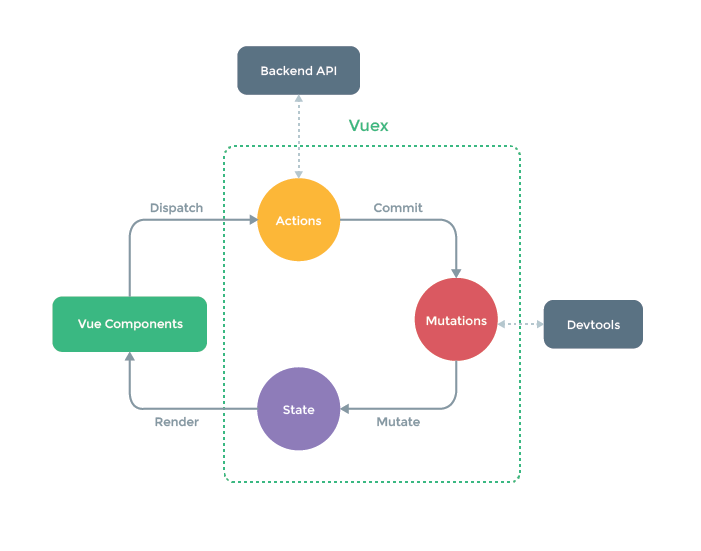
\includegraphics[width=1.25\textwidth]{vuex}
    \caption{Vuex Action-Mutations-State Diagram}
    \label{fig:mesh1}
\end{figure}

Komponenten k\"onnen auch private Zust\"ande haben, dies wird mit "privateState" erreicht. In diesem Fall muss der sharedState ebenfalls definiert werden.

\begin{figure}[H]
    \centering
    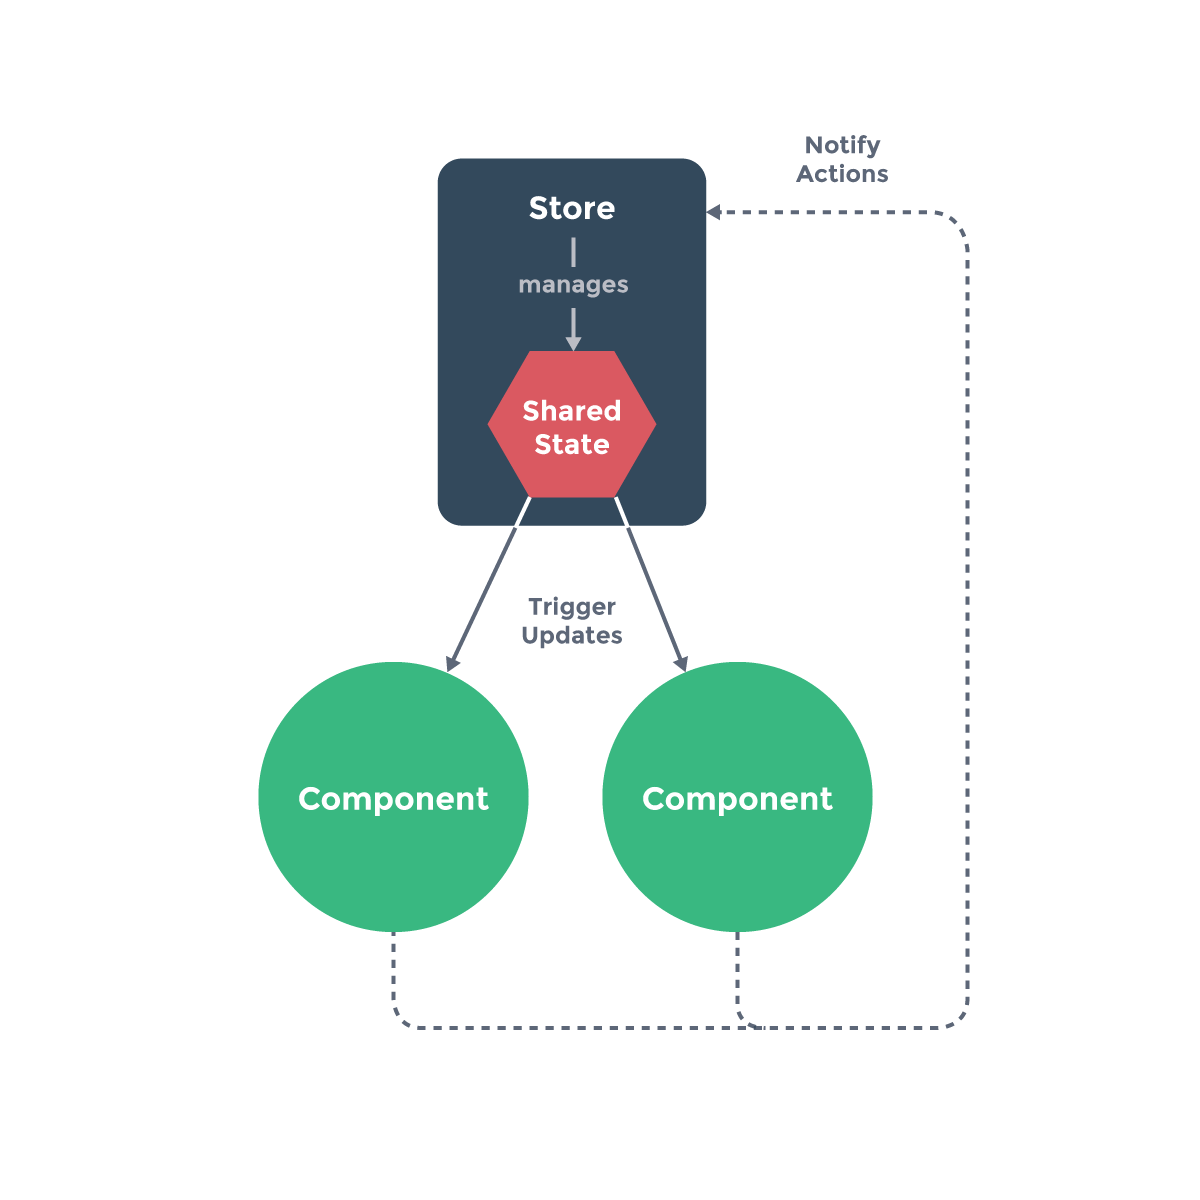
\includegraphics[width=1.25\textwidth]{sharedstate}
    \caption{Vuex private}
    \label{fig:mesh2}
\end{figure}

Dies bewirkt, dass eine Komponente nicht direkt einen Wert oder Zustand im Store ver\"andern kann, sondern dies einen Event aufruft. Dieser informiert den Store welchen State es \"uber eine Mutation zu ver\"andern gilt.


\section{Design}
\subsection{Architektur}
\subsection{Objektkatalog}
Waldstandort: Eine Fl�che auf der Erdoberfl�che, welche einen Walddarstellt $\newline$
Waldstandortstyp: Einer von vielen Typen, welcher einen Waldstandort einen bestimmten Typ zuordnet. Meist wird hier der K�rzel aus den Definitionen von ek72 verwendet, z.B. K�rzel "7e". Der volle Name des Waldstandortstyps "7e" ist "Waldmeister-Buchenwald mit Hornstrauch"
\subsection{Package Struktur}
Der Source-Code von "Waldmeister-Outdoors" ist auf GitHub unter "https://github.com/dschmide/Waldmeister-Outdoors" erh�tlich. Die Paket-Struktur des Projekts ist in die Teile "backen", "client", "Dokumentation" und "secured-local-nginx" aufgeteilt.
$\newline$
screenshots

\subsection{Sequenz-Diagramm}
\subsection{UI Design}
\subsubsection{Mockups}
Die Mockups wurden vor der Implementation erstellt, um Screendesign und Layout klarer zu definieren, bevor es um die technische Implementation von "Waldmeister - Outdoors" ging. In den Abbildungen 1 bis 9 kann man den Arbeitsschritt Einloggen und Erstellen einer neuen Fl\"ache und eines Points of Interests (POI) sehen. Zus\"atzlich sieht der User seine eigene Location auf der Map eingetragen und hat \"uber das Menu "My Places" Zugriff auf eine Liste seiner erstellten Fl\"achen. Ein Kontextmenu gibt bei der Anzeige eines ausgew\"ahlten Objekts zus\"atzliche Informationen.

\pagebreak

\begin{figure}[H]
\centering
    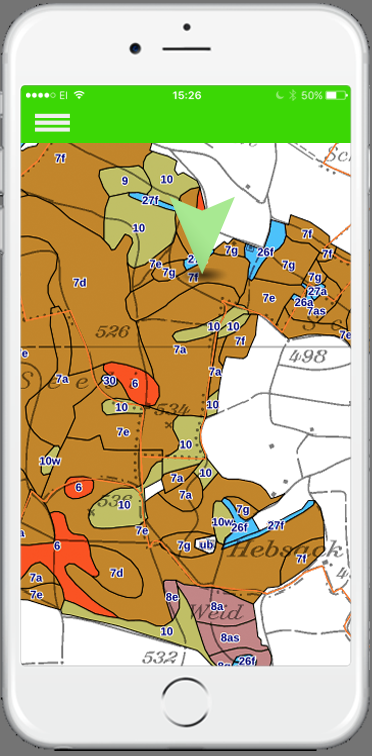
\includegraphics[width=0.7\textwidth]{mockup1-1}
    \caption{Mockup Screen 1}
    \label{fig:mesh1}
\end{figure}

\begin{figure}[H]
\centering
    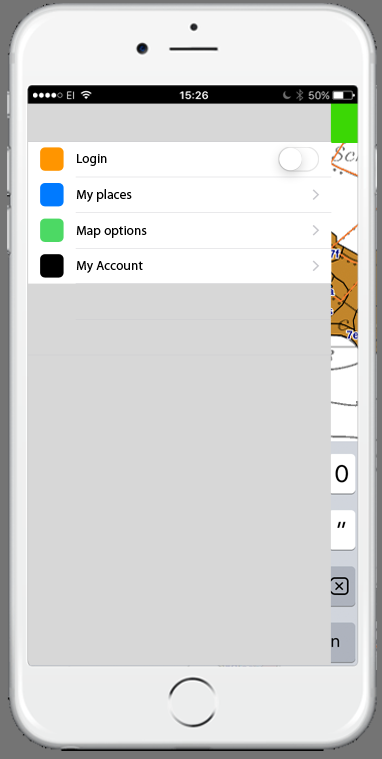
\includegraphics[width=0.7\textwidth]{mockup1-2}
    \caption{Mockup Screen 2}
    \label{fig:mesh2}
\end{figure}

\begin{figure}[H]
\centering
    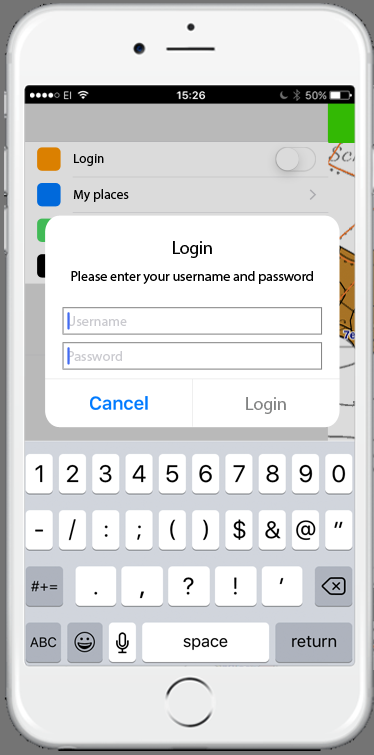
\includegraphics[width=0.7\textwidth]{mockup1-3}
    \caption{Mockup Screen 3}
    \label{fig:mesh3}
\end{figure}

\begin{figure}[H]
\centering
    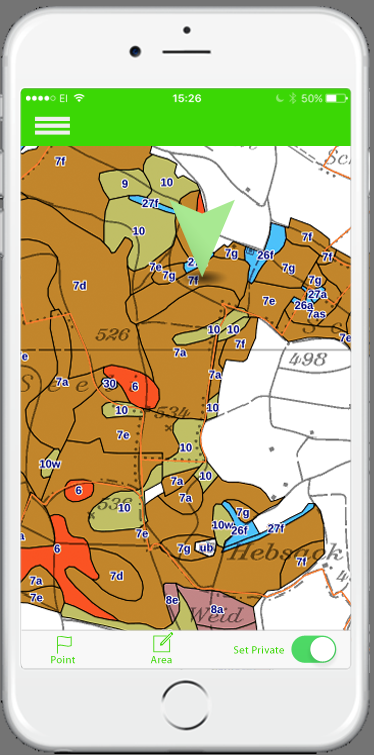
\includegraphics[width=0.7\textwidth]{mockup1-4}
    \caption{Mockup Screen 4}
    \label{fig:mesh4}
\end{figure}

\begin{figure}[H]
\centering
    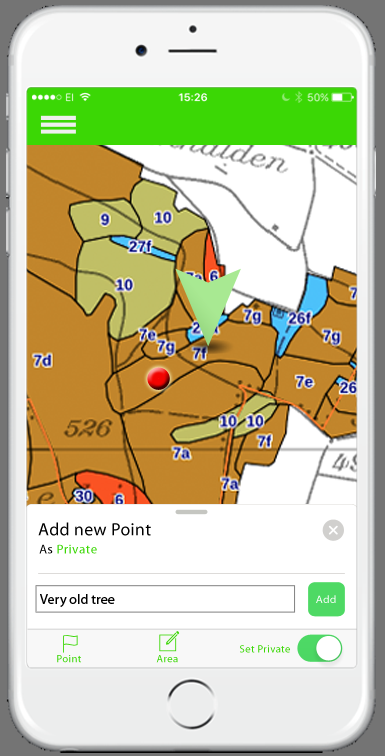
\includegraphics[width=0.7\textwidth]{mockup1-5}
    \caption{Mockup Screen 5}
    \label{fig:mesh5}
\end{figure}

\begin{figure}[H]
\centering
    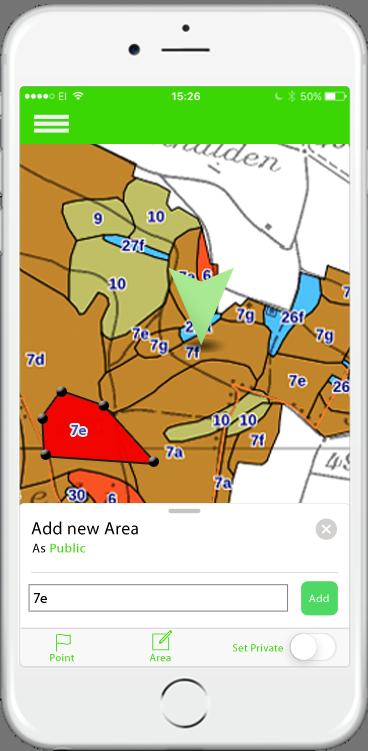
\includegraphics[width=0.7\textwidth]{mockup1-6}
    \caption{Mockup Screen 6}
    \label{fig:mesh6}
\end{figure}

\begin{figure}[H]
\centering
    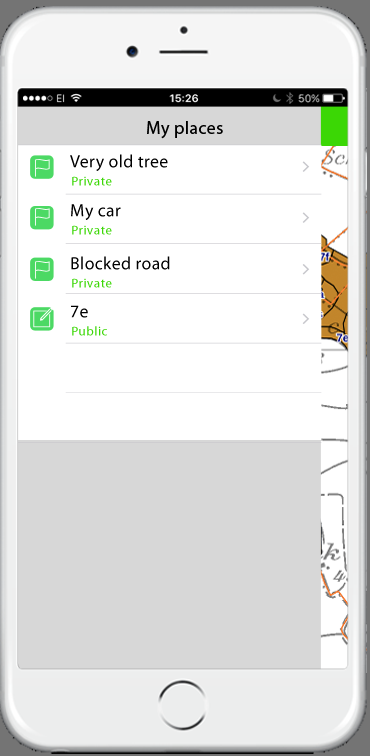
\includegraphics[width=0.7\textwidth]{mockup1-7}
    \caption{Mockup Screen 7}
    \label{fig:mesh7}
\end{figure}

\begin{figure}[H]
\centering
    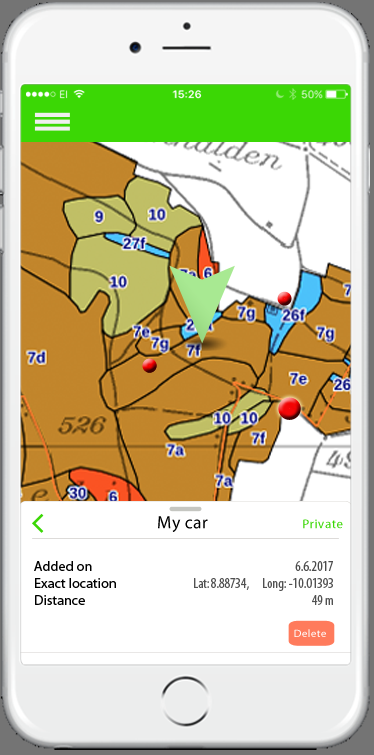
\includegraphics[width=0.7\textwidth]{mockup1-8}
    \caption{Mockup Screen 8}
    \label{fig:mesh8}
\end{figure}

\begin{figure}[H]
\centering
    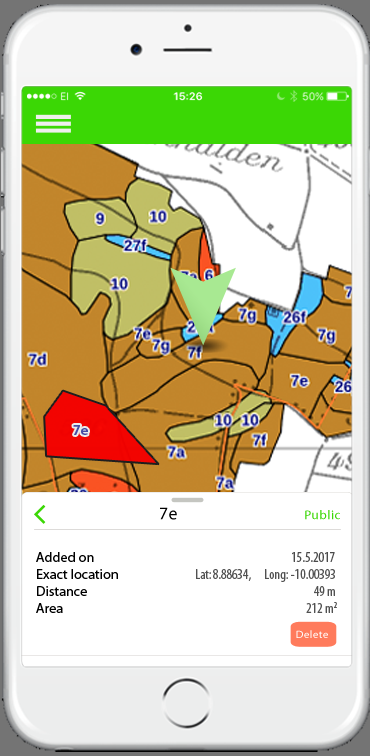
\includegraphics[width=0.7\textwidth]{mockup1-9}
    \caption{Mockup Screen 9}
    \label{fig:mesh9}
\end{figure}

\section{Implementation und Test}
\subsection{Implementation}
\subsubsection{Technische Implementation}
\subsubsection{API und Datenquellen}
\subsubsection{Login}
\subsubsection{Kartenmaterial}
\subsubsection{etc.}

\section{Automatische Testverfahren}
Testgetriebene Entwicklung (TDD) ist eine Methode zur Softwareentwicklung, welche oft bei der agilen Entwicklung von Computerprogrammen eingesetzt wird. Bei TDD erstellt der Programmierer Software-Tests, um das korrekte Verhalten von Softwarekomponenten zu planen und zu \"uberpr\"ufen. Unit Tests (auch als Unittest oder als Komponententest bezeichnet), werden verwendet um die funktionalen Einzelteile eines Softwareprojekts zu pr\"ufen. 

\subsection{Jasmine}
\subsection{Karma}
Tests f\"ur Vue.JS wurden mit dem Test Runner Karma und dem Testframework Jasmine erstellt . Sie k\"onnen \"uber den Befehl "npm run test" ausgef\"uhrt werden, aus dem "client" folder des Vue-Servers. $\newline$
Getestet werden Komponenten und deren Inhalt, welche von VueJS verwendet werden. $\newline$
Damit Jasmin die Tests ausf\"uhren kann, muss der Code von Webpack zuerst kompiliert werden. Danach wird er in einer Browserumgebung (z.B Chrome oder Firefox) ausgef\"uhrt und das Testframework sammelt die zu testenden Werte und Verhalten. Es vergleicht diese mit gegebenen Werten und Zust\"anden, welche vom Programmierer erwartet werden. Stimmen sie \"uberein, ist der Test bestanden. Stimmen sie nicht \"uberein, ist der Test gescheitert und Jasmine meldet einen Fehler.

\subsection{Travis}
\subsubsection{Continuous Integration}
Um Continuous mit automated build und testing zu realisieren, habe ich Travis verwendet. Die Software Travis CI wurde 2011 in Berlin erstellt und 2013 ver\"offentlicht. Auf der Website travis-ci.org wird das Repo, welches auf Github gehostet wird, verkn\"upft. Jedes mal wenn auf das remote Repo gepusht wird, f\"uhrt Travis die config in Form einer .yaml Datei aus, welche im root folder des Repos hinterlegt ist. Sie installiert alle Programme und Dependancies auf einer Linux Maschine und testet ob der Build in der aktuellen Version funktioniert. Es entsteht eine Version History mit dazugeh\"orender config. Travis meldet, ob der Build und die Tests erfolgreich durchgef\"uhrt werden konnten. Dies geschieht auch auf separaten Branches des Projekts.

\begin{figure}[H]
    \centering
    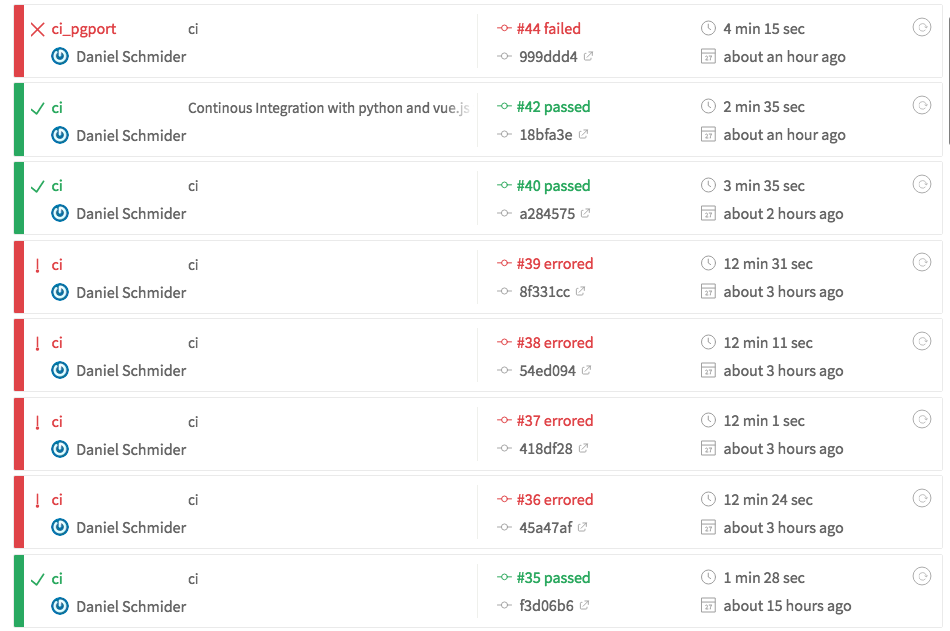
\includegraphics[width=1\textwidth]{travisv}
    \caption{TravisCI Version History}
    \label{fig:t1}
\end{figure}

\begin{figure}[H]
    \centering
    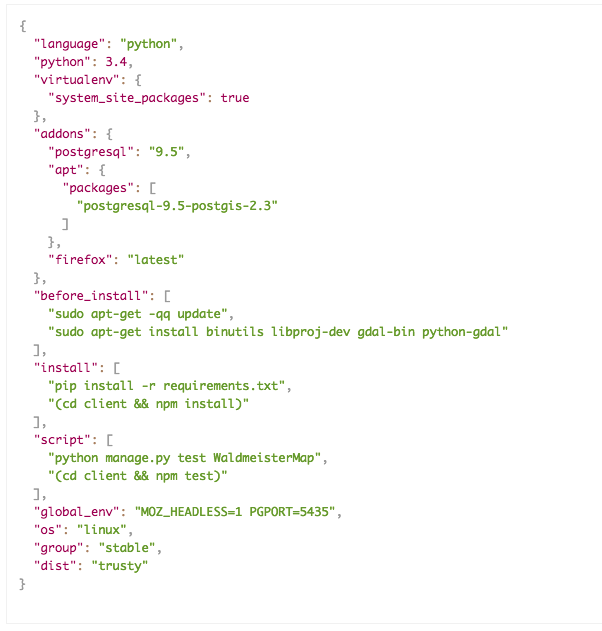
\includegraphics[width=1\textwidth]{travisc}
    \caption{Travis config .yaml, Version #45}
    \label{fig:t2}
\end{figure}

\begin{figure}[H]
    \centering
    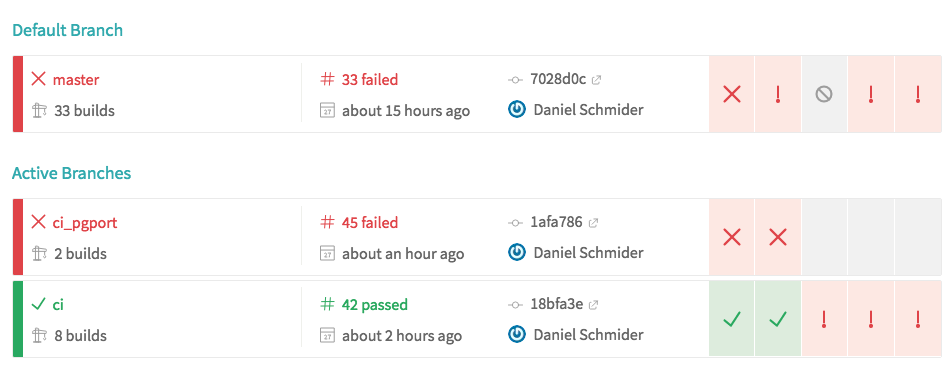
\includegraphics[width=1\textwidth]{travisb}
    \caption{Travis branches}
    \label{fig:t3}
\end{figure}

\section{Manuelle Tests}
\subsection{User-Szenario}
Das User-Szenario ist ein m�glicher Interaktionsablauf eines Users, welcher die Webapp "Waldmeister-Outdoors" verwendet. Es ist in die verschiedenen Schritte eingeteilt, welcher der User durchf�hrt.

1. Aufrufen der URL $\newline$
2. Scrollen, Zoomen der Map auf einen beliebigen Bereich $\newline$
3. Aufruf der "About" Seite $\newline$
4. �ffnen der Map-Legende in einem separaten Tab $\newline$
5. Registrierung eines neuen Users, Eingabe von Benutzernamen und Passwort $\newline$
6. Login mit dem neu erstellten Benutzers $\newline$
7. Erstellung einer neuen privaten Benutzerfl�che $\newline$
8. Updaten der gerade erstellten Benutzerfl�che $\newline$
9. Erstellen einer neuen �ffentlicher Benutzerfl�che $\newline$
10. Erstellen einer zweiten �ffnentlicher Benutzerfl�che $\newline$
11. L�schen einer erstellten Benutzerfl�che $\newline$
12. Ausloggen des Benutzers $\newline$
13. Registrierung eines zweiten Benutzers $\newline$
14. Einloggen des zweiten Benutzers $\newline$
15. L�schungsversuch einer �ffentlichen Benutzerfl�che, welche vom ersten Nutzer erstellt wurde $\newline$
16. Erstellen einer �ffentlichen Benutzerfl�che $\newline$
17. Updaten der erstellen Benutzerfl�che, wechseln des Labels und �ffentlich auf privat $\newline$

\subsection{Testf�lle}
Testfall A: $\newline$
Aufruf der URL $\newline$
Erwartet: Laden der Webapp$\newline$
Erf�llt: Ja/Nein$\newline$
$\newline$
Testfall B:$\newline$
Scrollen und Zoomen der Map$\newline$
Erwartet: Map scrollt durch drag & drop, zoomen durch Mousewheel oder Zoom Buttons
Erf�llt: Ja/Nein


\subsection{Ziel}

\subsection{Reproduktion}

\section{Resultate und Weiterentwicklung}
\subsection{Resultate}
\subsection{M�glichkeiten der Weiterentwicklung}
\subsection{Vorgehen}

\section{Projektmanagement}
\subsection{Allgemeines}
\subsubsection{GitHub}

\subsection{Meilensteinplanung}
Meilensteine beschreiben Wichtige geplante Daten im Projektablauf. Im Projekt "Waldmeister-Outdoors" gibt es folgende Meilensteine:

1. Projektplan erstellen 18.4. $\newline$
2. Refactoring der Codebase, 2.5.$\newline$
3. Feature Freeze / Feature Demo 23.5. $\newline$
4. Abgabe Projekt 8.6. $\newline$

\subsection{Releases}
Als Release wird das Deployment der Webapp auf den Produktions Server bezeichnet. Grunds�tzlich wird die Webapp auf einem Lokalen Testserver entwickelt und getestet. Bei einem Release wird die Lauff�hige Webapp auf das Livesystem portiert und �ffentlichen Usern zug�nglich gemacht.
\subsection{Issues}
W�hrend dem Projekt und insbesondere w�hrend der Projektplanungsphase werden Issues erfasst, welche geplante Schritte, Funktionen oder Arbeitsschritte beschreiben.
\subsection{Prototypen}
\subsection{Prozessmodell}
\subsubsection{Scrum}


\subsection{Aufwandsch�tzung}
\subsubsection{Zeitplan}
\subsubsection{Projektplan}

\subsection{Risiken}
\subsubsection{Deadlines}
\subsubsection{Technologien}
\subsubsection{Frameworks}
\subsubsection{Mobile Limits}

\section{Projektmonitoring}
\subsection{Soll-Ist-Zeitvergleich}
\subsection{Code Statistics}

\section{Softwaredokumentation}
\subsection{Installation}
\subsection{Tutorial, Handbuch}
\subsection{Referenzhandbuch}








% \input{chapter/04mychapter}
% ...


% List of figures & glossary
%%%%%%%%%%%%%%%%%%%%%%%%%%%%
\listoffigures
%\printglossary[type=\acronymtype,title=Abk�rzungsverzeichnis,style=long]

%\printglossary[type=\acronymtype]
\pagebreak
\Huge
Glossar
$\newline$

\Large
$\newline$
Akronyme$\newline$
\small
$\newline$
SRID = Spatial Reference Identifier
$\newline$ $\newline$
GIS = Geografisches Informationssystem
$\newline$ $\newline$
MVC = Model - View - Controller
$\newline$ $\newline$
MVVM = Model - View - ViewModel
$\newline$ $\newline$
HTML = Hypertext Markup Language
$\newline$ $\newline$
CSS = Cascading Style Sheets
$\newline$ $\newline$
ES5 = ECMA Script 5
$\newline$ $\newline$
ECMA = European Computer Manufacturers Association
$\newline$ $\newline$
SoC = Separation of Concern
$\newline$ $\newline$
SPA = Single-Page-Applikation
$\newline$ $\newline$
EK72 = Ellenberg Kl\"otzli
$\newline$ $\newline$
POI = Points of Interests
$\newline$ $\newline$
UML = Unified Modeling Language
$\newline$ $\newline$
JWT = (JSON Web Token)
$\newline$ $\newline$
JSON = JavaScript Object Notation
$\newline$ $\newline$
REST = Representational state transfer
$\newline$ $\newline$
CRUD = Create, Read, Update, Delete 
$\newline$ $\newline$
DRF = Django Rest-Framework
$\newline$ $\newline$
CI = Continuous Integration
$\newline$ $\newline$




% Bibliography
%%%%%%%%%%%%%%
\bibliographystyle {alpha}
\bibliography{index/bibliography}


% Attached sources
%%%%%%%%%%%%%%%%%%
%postgresql.conf



\end{document}